
%(BEGIN_QUESTION)
% Copyright 2008, Tony R. Kuphaldt, released under the Creative Commons Attribution License (v 1.0)
% This means you may do almost anything with this work of mine, so long as you give me proper credit

Calculate the proper $C_v$ value for a control valve used to control liquid level in a tank.  A guided-wave radar level transmitter measures the level of the liquid in the tank, and a controller throttles the valve to maintain that liquid level at approximately 25 feet above the centerline of the valve piping.  Assume a maximum valve flow rate of 350 GPM, and water as the process liquid:

$$\includegraphics[width=15.5cm]{i03220x01.eps}$$

Also, calculate the approximate pipe size of control valve necessary to achieve this flow capacity, assuming the use of a characterized ball valve ($C_d$ = 25).

\vskip 10pt

Now, re-calculate both the $C_v$ and valve pipe size, assuming the process liquid is kerosene (density = 51.2 lb/ft$^{3}$) instead of water.  Does this change require a larger valve, a smaller valve, or will the same valve size work for kerosene as it did for water?  Explain your answer.

\vskip 20pt \vbox{\hrule \hbox{\strut \vrule{} {\bf Suggestions for Socratic discussion} \vrule} \hrule}

\begin{itemize}
\item{} Suppose the control valve discharged liquid to a line with a constant pressure of 4 PSI instead of discharging to atmospheric pressure.  How would this change affect the necessary sizing of the control valve?
\item{} Based on what you see here, will this process exhibit a {\it self-regulating}, {\it integrating}, or {\it runaway} characteristic?
\item{} Identify in qualitative terms how you would expect to have to tune the level controller in this system.  Would you expect to use aggressive proportional action, integral action, and/or derivative action?  Are there certain control actions such as derivative you would {\it not} with to use in this loop?  Explain your reasoning.
\item{} For those who have studied liquid level measurement, explain how a {\it radar} level transmitter senses liquid level in the process vessel.
\item{} Suppose this loop-powered radar level transmitter were replaced by one that was wireless, powered by a battery instead of by 24 VDC loop power.  Such transmitters conserve battery power by reporting the process variable infrequently.  Explain how this change may affect the quality of control for this process.
\end{itemize}

\underbar{file i03220}
%(END_QUESTION)





%(BEGIN_ANSWER)

The density of the liquid is irrelevant in this problem only because the differential pressure across the valve comes solely from hydrostatic head (gravity acting on the liquid) only.  Thus, the {\it same size valve} will work for kerosene as it will for water:

\vskip 10pt

$C_v$ = 106
 
\vskip 10pt

A 2.5 inch control valve should be sufficient.

\vskip 10pt

However, a different valve size would be required for kerosene if the pressure drop across the valve came from a pump rather than from gravity!

%(END_ANSWER)





%(BEGIN_NOTES)

$$Q = C_v \sqrt{\Delta P \over G_f}$$

$$\Delta P = \left(25 \hbox{ ft WC} \over 1 \right) \left(12 \hbox{ "} \over 1 \hbox{ ft} \right) \left(1 \hbox{ PSI} \over 27.68 \hbox{ "WC} \right) = 10.838 \hbox{ PSI}$$

$$C_v = {Q \over \sqrt{\Delta P \over G_f}} = {350 \over \sqrt{10.838 \over 1}} = 106.3$$

\vskip 10pt

$$C_d = {C_v \over d^2}$$

$$d^2 = {C_v \over C_d}$$

$$d = \sqrt{C_v \over C_d} = \sqrt{106.3 \over 25} = 2.062 \hbox{ inches diameter}$$

\vskip 10pt

$d$ = 2.062 inches, rounded up to 2.5 inches nominal.

\vskip 10pt

Kerosene, being less dense than water, will generate less hydrostatic head.  However, less hydrostatic head will be necessary to force the same flow rate through the valve, since $G_f$ is part of the valve sizing equation.  So, specific gravity ends up being irrelevant in this problem.

\vfil \eject

\noindent
{\bf Prep Quiz:}

Calculate the necessary $C_v$ for a control valve to flow 220 GPM of water at a pressure drop (across the valve) of 5.7 PSI:

\begin{itemize}
\item{} 92.15
\vskip 5pt 
\item{} 84.54
\vskip 5pt 
\item{} 1254
\vskip 5pt 
\item{} 38.60
\vskip 5pt 
\item{} 80.33
\vskip 5pt 
\item{} 2.602
\end{itemize}

%INDEX% Final Control Elements, valve: sizing

%(END_NOTES)


